\documentclass[10pt,a5]{article}

\usepackage{paracol}
%\usepackage[landscape]{geometry}
\usepackage[left=1.5cm, right=1.5cm, top = 2cm, bottom = 2cm]{geometry}
%\usepackage{pdfpages}
\usepackage{graphicx}
\usepackage{liturg}
\usepackage{lipsum}

\newcommand \sect[2] {\section*{#1} \switchcolumn \section*{#2} \switchcolumn*}
\newcommand \subsect[2] {\subsection*{#1} \switchcolumn \subsection*{#2} \switchcolumn*}

\setlength\parindent{0pt}

\begin{document}

\massenglish

%\psalmheading{Psalm 42---Judica me}

%\instruct{The priest, signing himself with the Sign of the Cross, says:}

%\leslettrine{C}onf'iteor Deo omnipot'enti, be'at"ae Mar'i"ae semper
%V'irgini, be'ato Micha'eli Arch'angelo, be'ato Jo'anni Bapt'ist"ae,
%sanctis Ap'ostolis Petro et Paulo, 'omnibus Sanctis, et tibi Pater:
%quia pecc'avi nimis congitati'one, verbo, et 'opere:

\begin{paracol}{2}

\sect{Introductory Rites}{Ritos Iniciais}

\subsect{Entrance}{Canto de Entrada}

\subsect{Greeting}{Acolhida}

%\switchcolumn

\priest{The Lord be with you}

\server{And with your spirit}

\switchcolumn

\padre{A graça de Nosso Senhor Jesus Cristo, o amor do Pai e a comunhão do Espírito Santo estejam convosco.}
\todos{Bendito seja Deus, que nos reuniu no amor de Cristo.}

\switchcolumn*

\subsect{Penitential Act}{Ato Penitencial}

\end{paracol}

\begin{figure}[h]
	\centering
	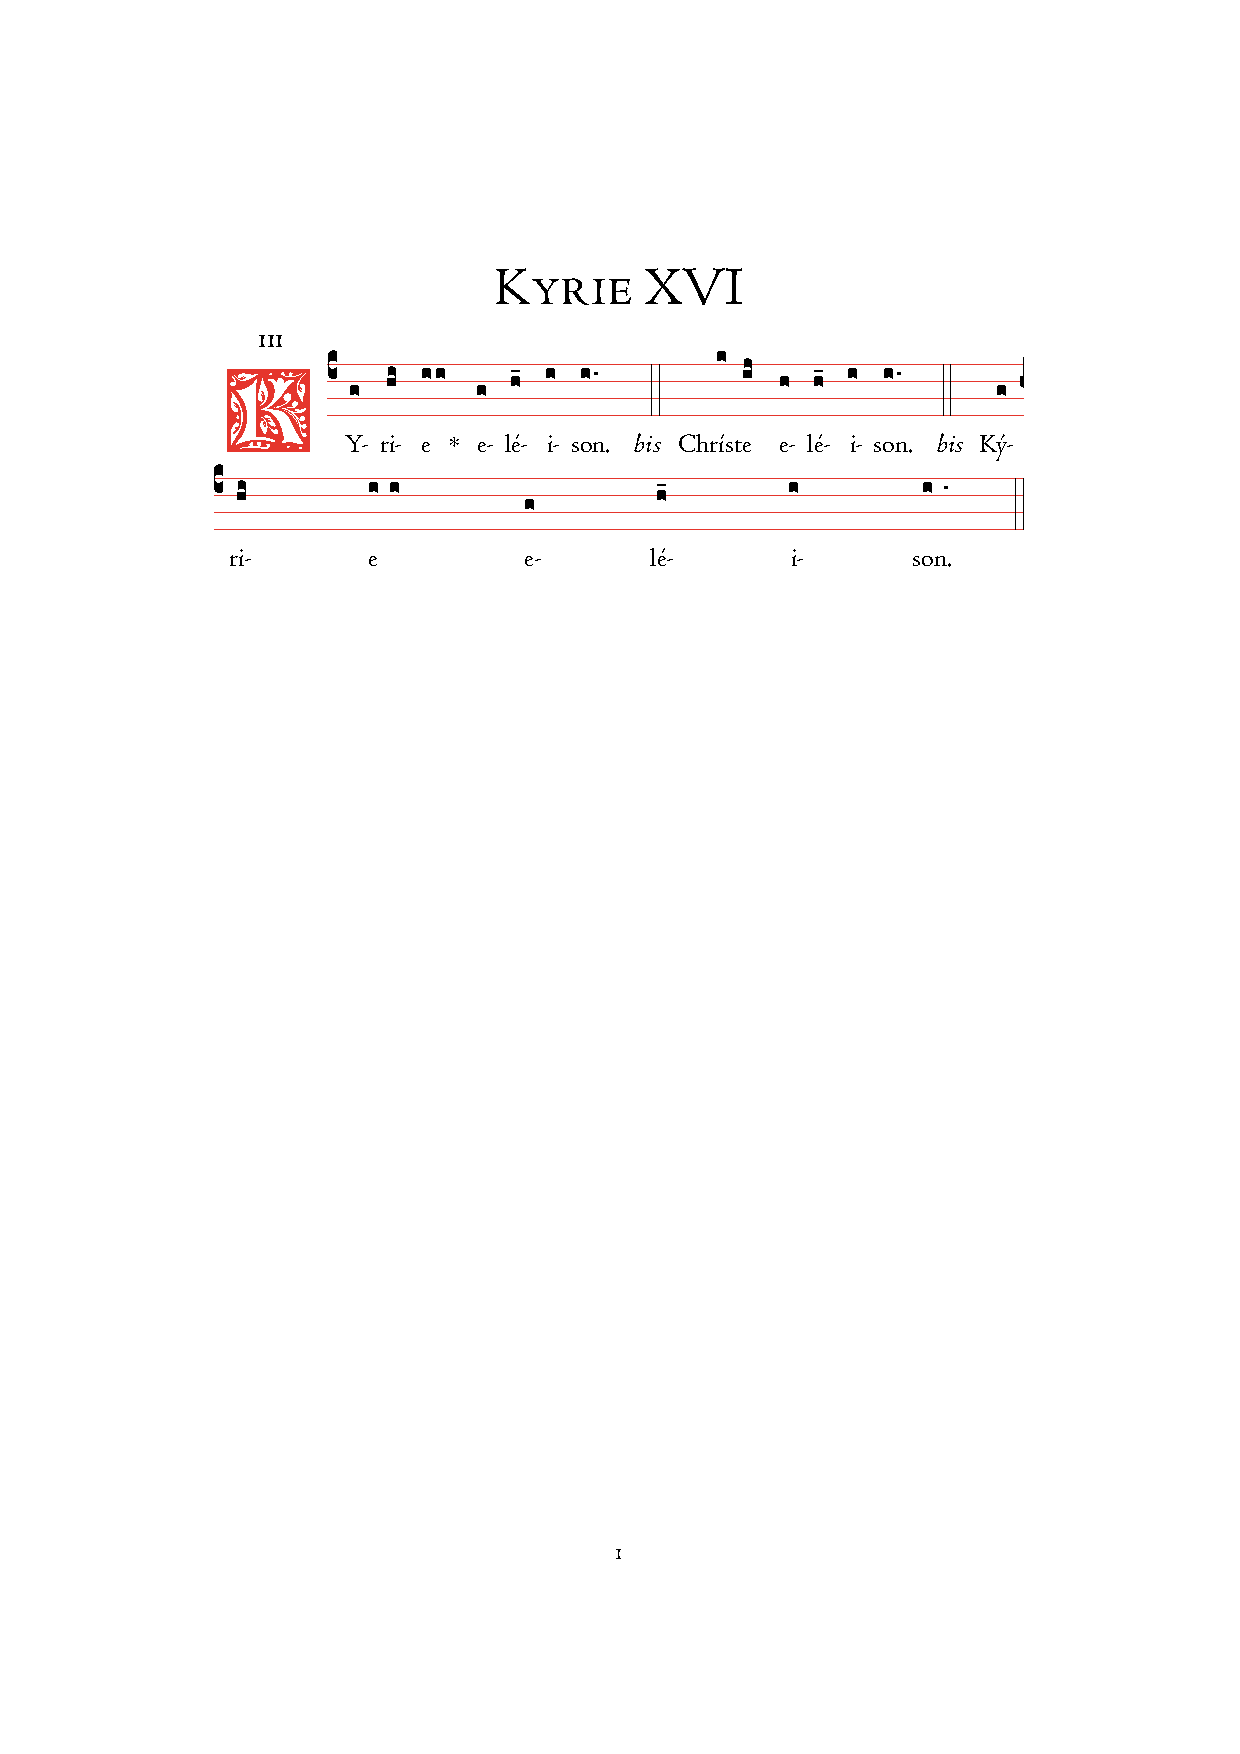
\includegraphics[trim = 35mm 200mm 35.5mm 45mm, clip, width = 0.8\textwidth]{scores/Kyrie-XVI.pdf}
\end{figure}

\begin{paracol}{2}

(Lord, have mercy. Christ, have mercy. Lord, have mercy.)
\switchcolumn
(Senhor, tende piede. Cristo, tende piedade. Senhor, tende piedade)

\switchcolumn*

\subsect{Glory to God}{Gl\'oria}

\end{paracol}

\begin{figure}
	\centering
	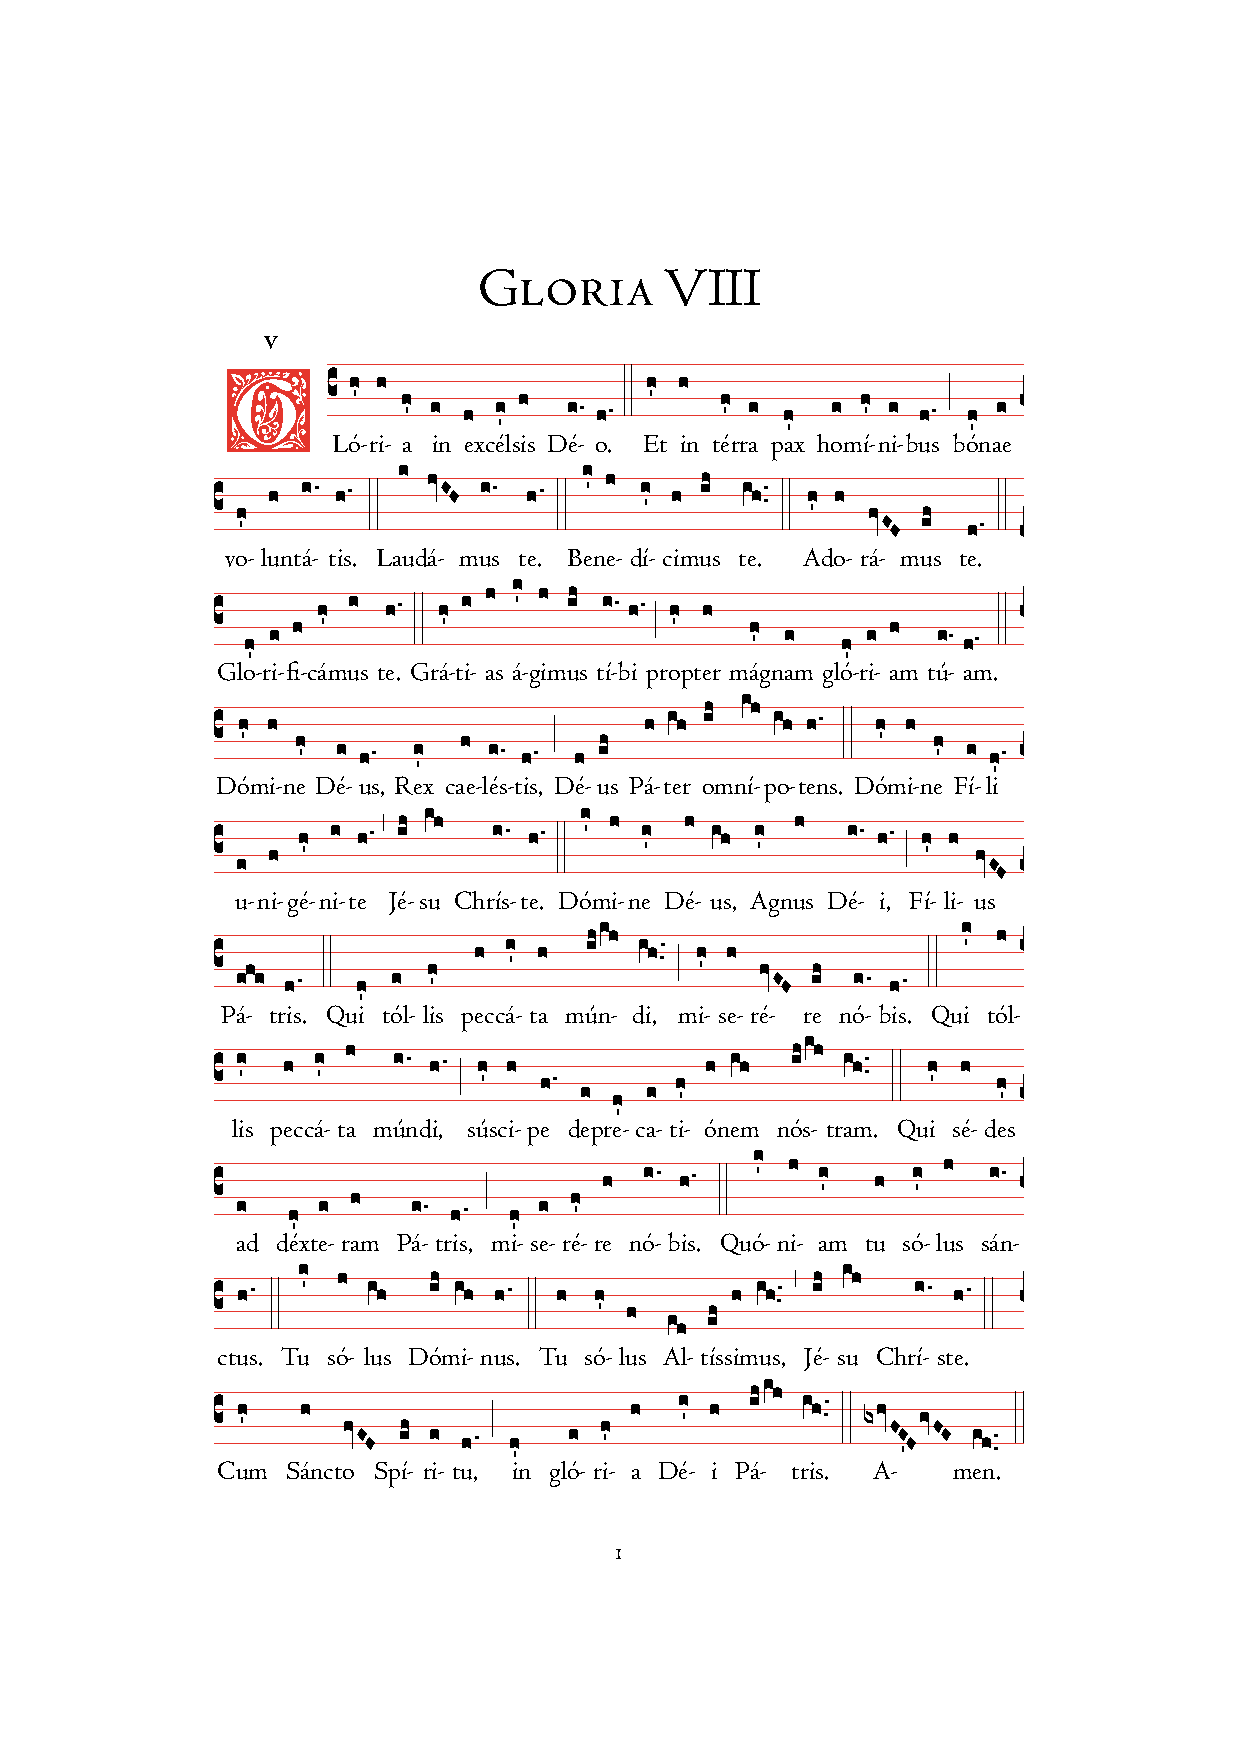
\includegraphics[trim = 35mm 45mm 35.5mm 45mm, clip, width = 0.8\textwidth]{scores/Gloria-VIII.pdf}
\end{figure}

\begin{paracol}{2}

(Glory to God in the highest,
and on earth peace to people
of good will.
We praise you, we bless you,
we adore you, we glorify you,
we give you thanks for your great
glory,
Lord God, heavenly King, O God,
almighty Father.
Lord Jesus Christ, Only Begotten Son,
Lord God, Lamb of God, Son of the
Father,
you take away the sins of the world,
have mercy on us;
you take away the sins of the world,
receive our prayer;
you are seated at the right hand
of the Father, have mercy on us.
For you alone are the Holy One,
you alone are the Lord,
you alone are the Most High,
Jesus Christ, with the Holy Spirit,
in the glory of God the Father. Amen.)

\switchcolumn

(Gl\'oria a Deus nas alturas e paz na terra aos homens por Ele amados.
 Senhor Deus, Rei dos c\'eus, Deus Pai todo-poderoso:
 n\'os Vos louvamos, n\'os Vos bendizemos, n\'os Vos adoramos, n\'os Vos glorificamos,
 n\'os Vos damos graças, por vossa imensa gl\'oria.
 Senhor Jesus Cristo, Filho Unig\'enito, Senhor Deus, Cordeiro de Deus, Filho de Deus Pai:
 V\'os que tirais o pecado do mundo, tende piedade de n\'os;
 V\'os que tirais o pecado do mundo, acolhei a nossa s\'uplica;
 V\'os que estais \`a direita do Pai, tende piedade de n\'os.
 S\'o V\'os sois o Santo;
 s\'o V\'os, o Senhor;
 s\'o V\'os, o Alt\'issimo, Jesus Cristo;
 com o Esp\'irito Santo na gl\'oria de Deus Pai.
 Am\'em)

 \switchcolumn*

 \sect{Litugy of the Word}{Liturgia da Palavra}

 \sect{First Reading}{Primeira Leitura}

 %\lipsum[3]

 \server{Thanks be to God!}

 \switchcolumn

 %\lipsum[3]

 \todos{Gra\c{c}as a Deus!}

 \switchcolumn*

 \subsect{Responsorial Psalm}{Salmo Responsorial}

 %\lipsum[1]

 \switchcolumn

 %\lipsum[1]

 \switchcolumn*

 \subsect{Second Reading}{Segunda Leitura}

 %\lipsum[3]

 \server{Thanks be to God.}

 \switchcolumn

 %\lipsum[3]

 \todos{Gra\c{c}as a Deus!}

 \switchcolumn*

 \subsect{Gospel}{Evangelho}

 %\lipsum[3]

 \server{Glory to you O Lord.}

 \switchcolumn

 %\lipsum[3]

 \todos{Gl\'oria a v\'os, Senhor!}

 \switchcolumn*

 \subsect{Homily}{Homilia}

 \subsect{The Creed}{Profiss\~ao de f\'e}
I believe in one God,\\
the Father almighty,\\
maker of heaven and earth,\\
of all things visible and invisible.\\

\noindent
I believe in one Lord Jesus Christ,\\
the Only Begotten Son of God,\\
born of the Father before all ages.\\
God from God, Light from Light,\\
true God from true God,\\
begotten, not made,\\
consubstantial with the Father;\\
through him all things were made.\\
For us men and for our salvation\\
he came down from heaven,\\
{\tiny\textit{ At the words that follow, up to and including and became man, all bow.}}\\
and by the Holy Spirit was incarnate\\
of the Virgin Mary,\\
and became man.\\
For our sake he was crucified\\
under Pontius Pilate,\\
he suffered death and was buried,\\
and rose again on the third day\\
in accordance with the Scriptures.\\
He ascended into heaven\\
and is seated at the right hand\\
of the Father.\\
He will come again in glory\\
to judge the living and the dead\\
and his kingdom will have no end.\\

\noindent
I believe in the Holy Spirit,\\
the Lord, the giver of life,\\
who proceeds from the Father\\
and the Son,\\
who with the Father and the Son\\
is adored and glorified,\\
who has spoken through the prophets.\\

\noindent
I believe in one, holy, catholic\\
and apostolic Church.\\
I confess one Baptism\\
for the forgiveness of sins\\
and I look forward to the resurrection\\
of the dead\\
and the life of the world to come. Amen.\\
The Apostles’ Creed\\
I believe in God,\\
the Father almighty,\\
Creator of heaven and earth,\\
and in Jesus Christ, his only Son,\\
our Lord,\\
{\tiny At the words that follow, up to and including the Virgin Mary, all bow.}\\
who was conceived by the Holy Spirit,\\
born of the Virgin Mary,\\
suffered under Pontius Pilate,\\
was crucified, died and was buried;\\
he descended into hell;\\
on the third day he rose again\\
from the dead;\\
he ascended into heaven,\\
and is seated at the right hand\\
of God the Father almighty;\\
from there he will come to judge\\
the living and the dead.\\
I believe in the Holy Spirit,\\
the holy catholic Church,\\
the communion of saints,\\
the forgiveness of sins,\\
the resurrection of the body,\\
and life everlasting. Amen.

\switchcolumn

%TODO
Credo Niceno-Constantinopolitano

\switchcolumn*

\subsect{Universal Prayer}{Ora\c{c}\~{a}o universal}
\small\textit{After each intention there is a pause while the faithful pray.}

\priest{... we pray}
\server{Lord, hear our prayer.}

\sect{The Liturgy of the Eucharist}{Liturgia Eucar\'{i}stica}

\subsect{Offertory}{Canto do Ofert\'orio}

\priest{Pray, brothers and sisters, that my sacrifice and yours may be acceptable to God, the almighty Father.}

\server{May the Lord accept the sacrifice at your hands for the praise and glory of his name, for our good and the good of all his holy Church.}

\small\textit{Then the Priest, with hands extended, says the Prayer over the Offerings.}

\priest{...through Christ, our Lord.}
\server{Amen.}

\subsect{Eucharystic Prayer}{Ora\c{c}\~{a}o Eucar\'{i}stica}
\priest{The Lord be with you.}
\server{And with your spirit. }
\priest{Lift up your hearts. }
\server{We lift them up to the Lord. }
\priest{Let us give thanks to the Lord our God. }
\server{It is right and just.}

\small{\textit{The Priest, with hands extended, continues the Preface. At the end, he joins his hands and concludes the Preface as follows:}}

\priest{...without end we acclaim:}
\end{paracol}

\begin{figure}[h]
	\centering
	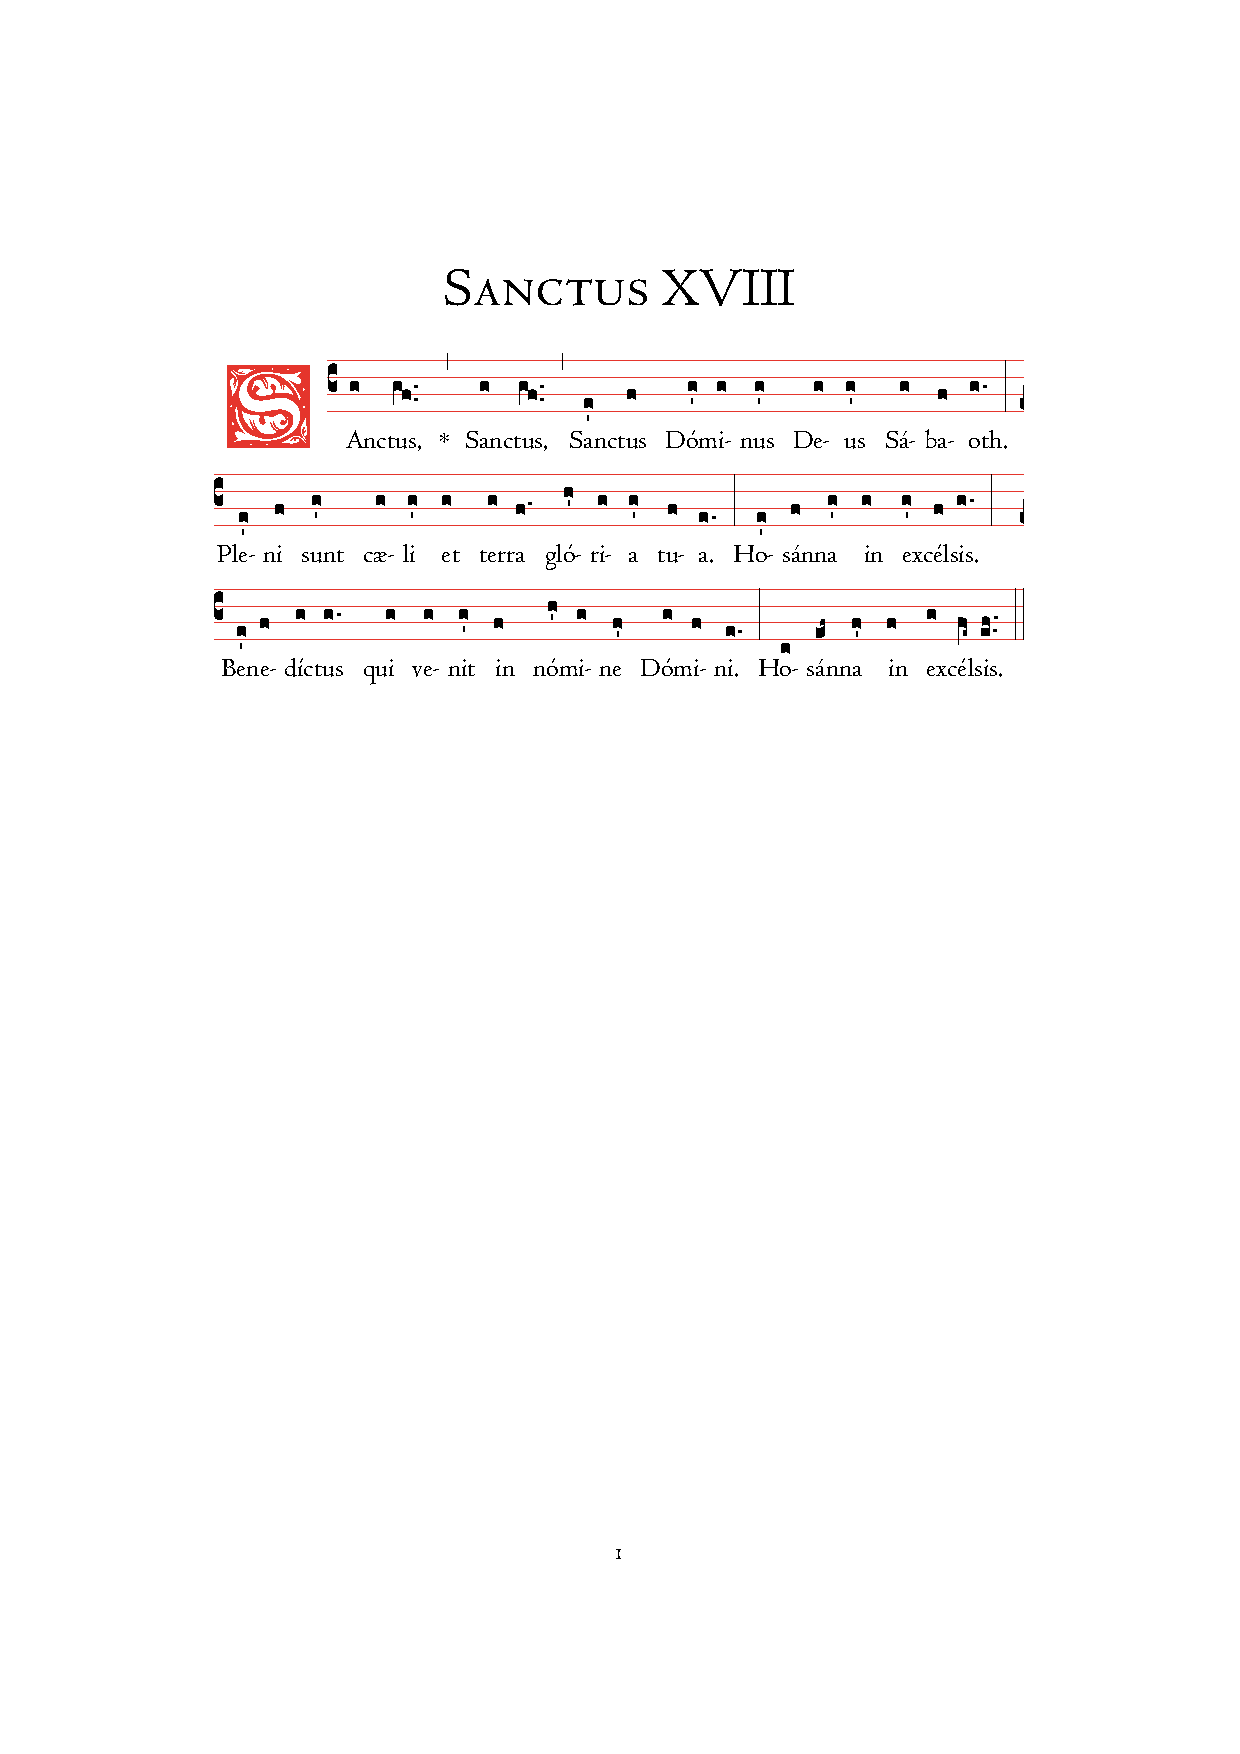
\includegraphics[trim = 35mm 175mm 35.5mm 45mm, clip, width = 0.8\textwidth]{scores/Sanctus-XVIII.pdf}
\end{figure}

\begin{paracol}{2}

(Holy, holy, holy lord God of hosts.
Heaven and earth are full of your glory.
Hosanna in the highest.
Blessed is he who comes in the name of the Lord.
Hosanna in the highest.)

\switchcolumn
Santo, santo, santo...

\switchcolumn*

\medskip 
\small{\textit{This is the high point of the Mass, where the bread and wine get changed into the Body and Blood of Christ.The Priest begins a prayer, and after the Priest holds up the bread and says the following words, bow as the Priest kneels.}}

\priest{TAKE THIS, ALL OF YOU, AND EAT IT:
THIS IS MY BODY WHICH WILL BE GIVEN UP FOR YOU.}

\small{\textit{The priest continues the prayer, and after the Priest holds up the cup and says the following words, bow as the Priest kneels.}}

\priest{TAKE THIS, ALL OF YOU, AND DRINK FROM IT:
THIS IS THE CUP OF MY BLOOD,
THE BLOOD OF THE NEW AND EVERLASTING COVENANT.
IT WILL BE SHED FOR YOU AND FOR ALL
SO THAT SINS MAY BE FORGIVEN.
DO THIS IN MEMORY OF ME.}

\priest{The mystery of faith}

\end{paracol}

\begin{figure}[h]
	\centering
	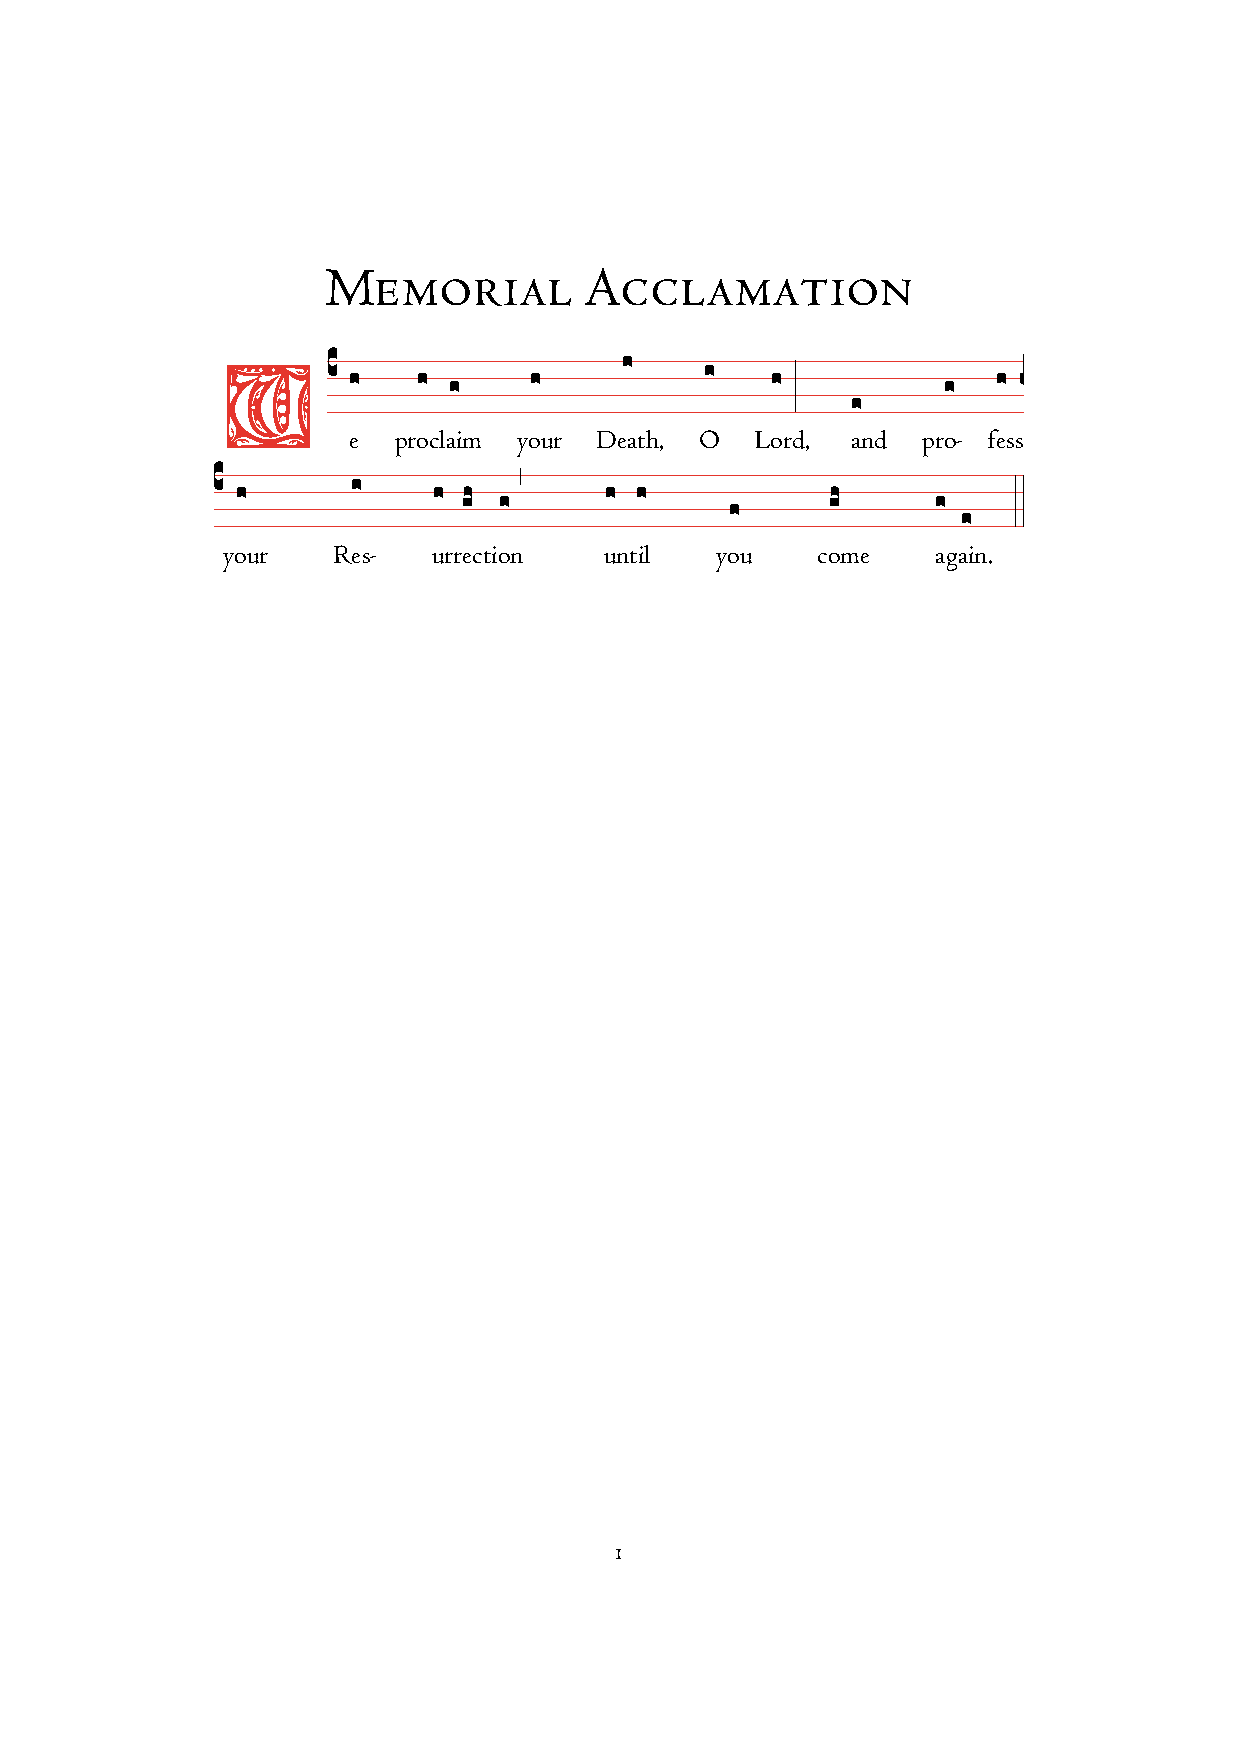
\includegraphics[trim = 35mm 195mm 35.5mm 45mm, clip, width = 0.8\textwidth]{scores/Memorial-Acclamation.pdf}
\end{figure}


%\greatfeast{Feria Quinta in Cena Domini}{I}

%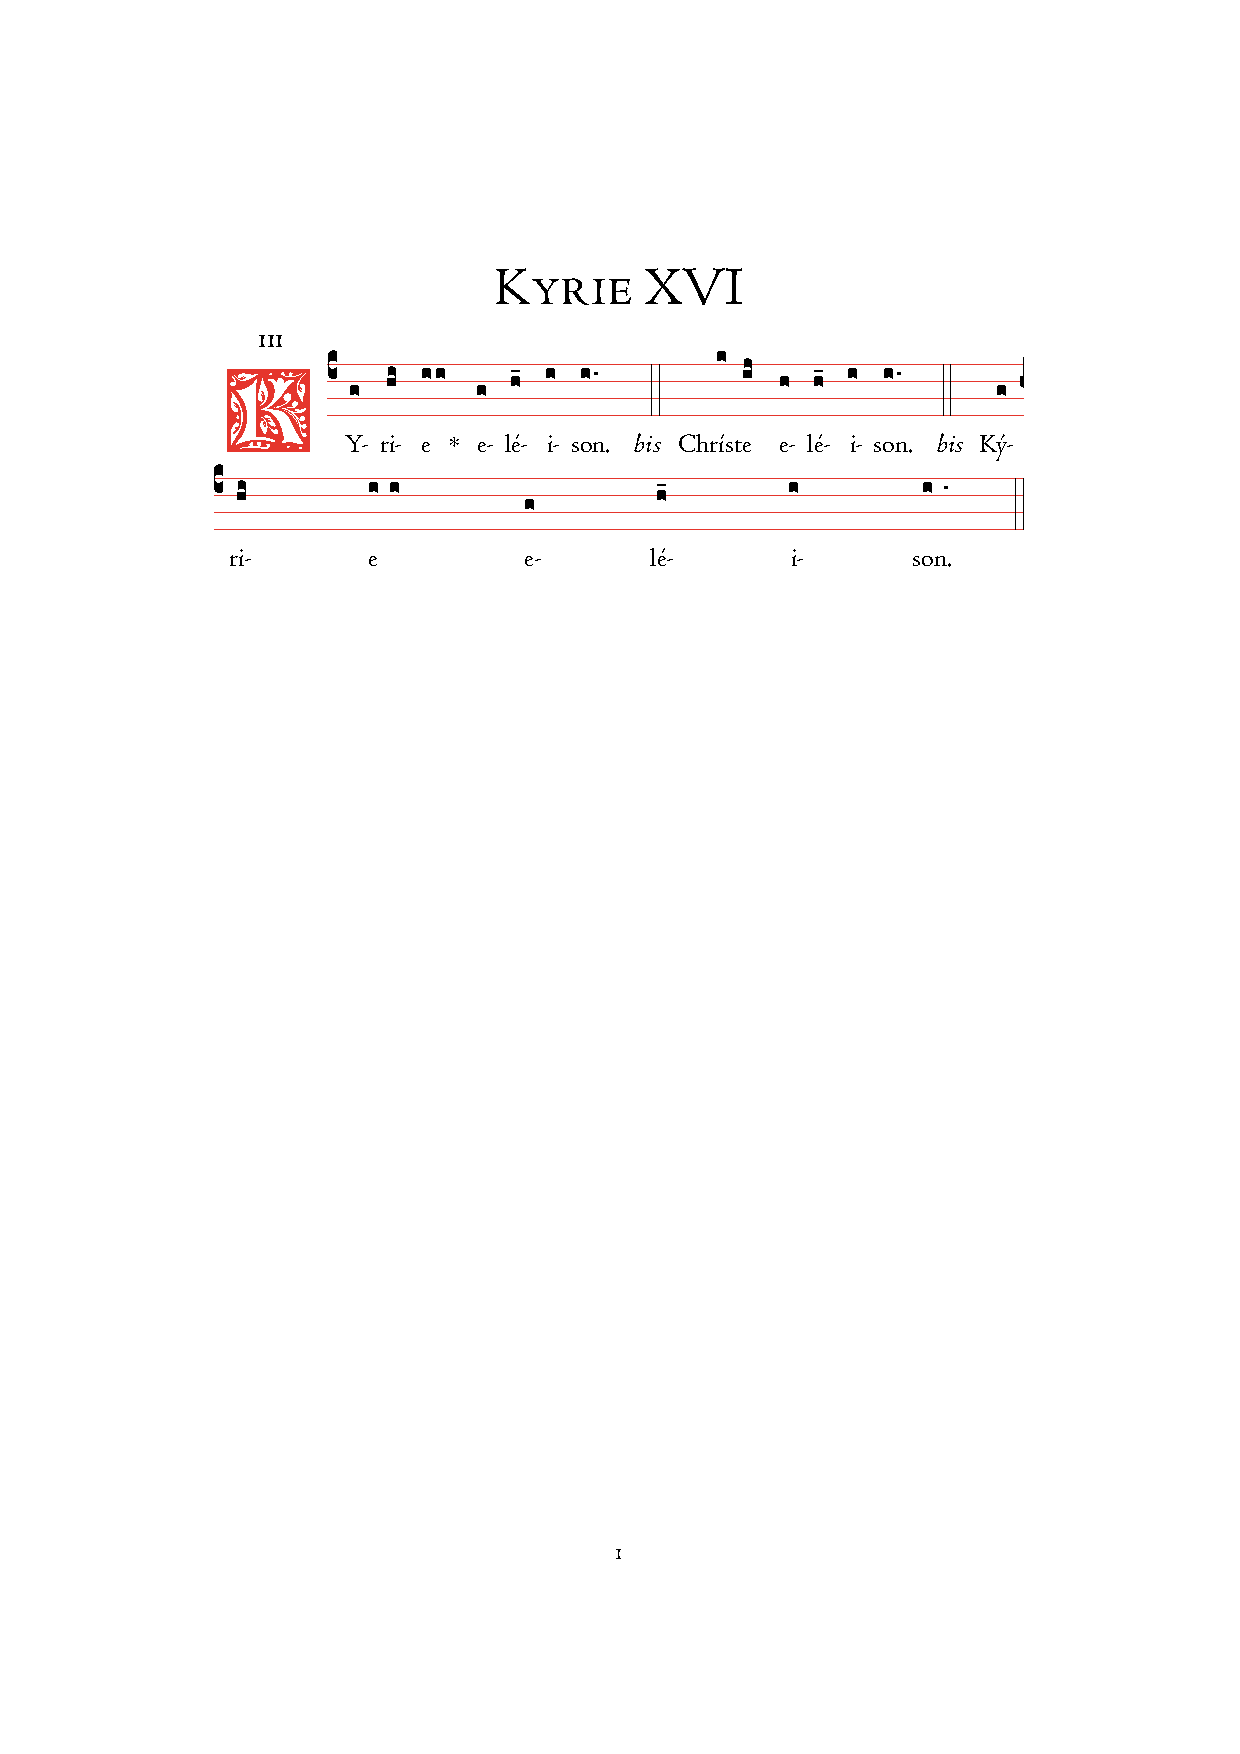
\includepdf[pages=-,pagecommand={},width=\textwidth, trim = 35mm 200mm 20mm 45mm, clip]{scores/Kyrie-XVI.pdf}
\end{document}
